\documentclass{CInf_practice}

\sheet{8}{Schaltwerke \& Register-Transfer-Ebene}
\usetikzlibrary{automata,positioning,arrows.meta,fit,shapes.misc}
\lstset{xleftmargin=0pt,xrightmargin=0pt,morekeywords={fi,declare,register,array,bus,memory,goto,then,read}}

\begin{document}
\cinftitle

\ex{Füllstandsregelung}{4 + 6 + 12 + 8 = 30}

\subex{Ein- \& Ausgangssignale, Modulbild}
\noindent Eingaben:
\begin{enumerate}[align=left,leftmargin=\marginparwidth]
   \item[$X_t$] Sensor oben (top), 1 = feucht, 0 = trocken
   \item[$X_m$] Sensor mitte (middle), 1 = feucht, 0 = trocken
   \item[$X_b$] Sensor unten (bottom), 1 = feucht, 0 = trocken
\end{enumerate}
Ausgaben:
\begin{enumerate}[align=left,leftmargin=\marginparwidth]
   \item[$Y$] Abflusssteuerung, 1 = öffnen, 0 = schließen
   \item[$E$] Errorsignal, 1 = Error, 0 = kein Error
\end{enumerate}

\tikzset{bus/.style 2 args={strike out,
                     draw,
                     -,
                     append after command={
                        node[#2=.1ex of \tikzlastnode] {\small #1}
                        }
                     }
        }
\begin{center}
  \begin{tikzpicture}
    % module
    \draw (2,3) rectangle node {Sicherheitsfüllstandregler (SFR)} +(6,-2);
    % in
    \draw[{Latex}-] (2,2.5) -- node[bus={1}{above}] {} ++(-1,0) node[left] {$X_t$};
    \draw[{Latex}-] (2,2) -- node[bus={1}{above}] {} ++(-1,0) node[left] {$X_m$};
    \draw[{Latex}-] (2,1.5) -- node[bus={1}{above}] {} ++(-1,0) node[left] {$X_b$};
    % out
    \draw[-{Latex}] (8,2) -- node[bus={1}{above}] {} ++(1,0) node[right] {$Y$};
  \end{tikzpicture}
\end{center}

\newpage
\subex{Zustandsgraph}

\begin{center}
  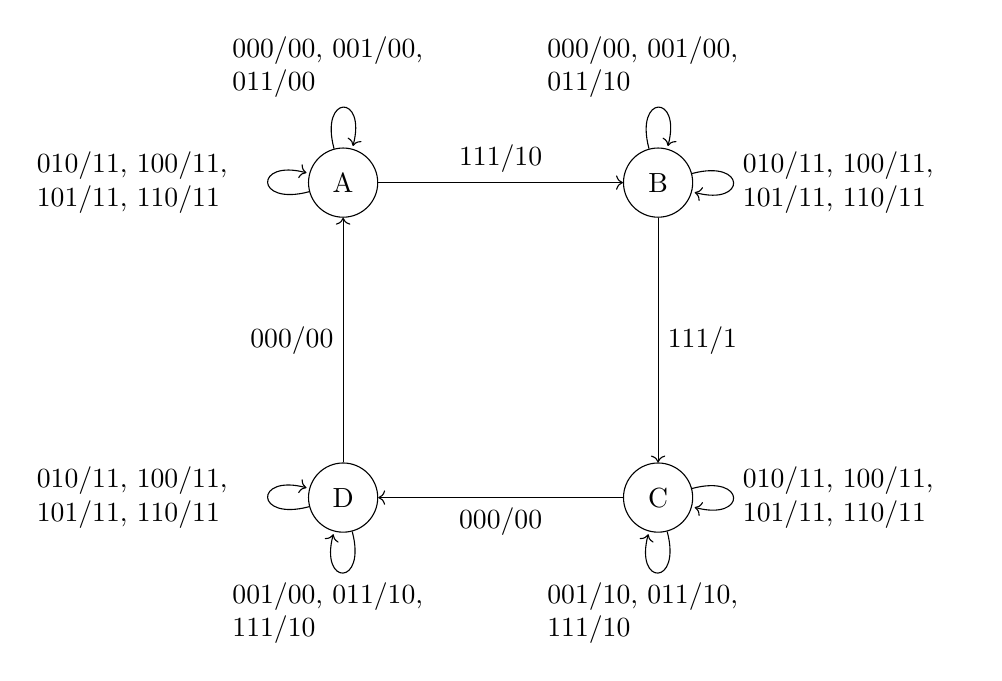
\begin{tikzpicture}[node distance=4cm]
    \node[state] (A) {A};
    \node[state,right of=A] (B) {B};
    \node[state,below of=B] (C) {C};
    \node[state,left of=C] (D) {D};
    
    \path[->] % inlet
              (A) edge[loop above] node[above, text width=8em] {000/00, 001/00, 011/00} (A) % valid
              (A) edge[loop left]  node[left, text width=8em]  {010/11, 100/11, 101/11, 110/11} (A) % error
              (A) edge             node[above]                 {111/10} (B) % next
  
              % hold it
              (B) edge[loop above] node[above, text width=8em] {000/00, 001/00, 011/10}(B) % valid
              (B) edge[loop right] node[right, text width=8em] {010/11, 100/11, 101/11, 110/11}(B) % error
              (B) edge             node[right]                 {111/1}(C) % next
              
              % outlet
              (C) edge[loop below] node[below, text width=8em] {001/10, 011/10, 111/10}(C) % valid
              (C) edge[loop right] node[right, text width=8em] {010/11, 100/11, 101/11, 110/11}(C) % error
              (C) edge             node[below]                 {000/00}(D) % next
              
              % hold it
              (D) edge[loop below] node[below, text width=8em] {001/00, 011/10, 111/10}(D) % valid
              (D) edge[loop left]  node[left, text width=8em]  {010/11, 100/11, 101/11, 110/11}(D) % error
              (D) edge             node[left]                  {000/00}(A) % next
              ;
              
  \end{tikzpicture}
\end{center}
\begin{center}
  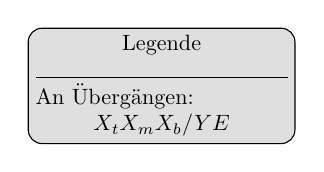
\begin{tikzpicture}
    \node[scale=.8,draw,rounded corners=5pt,fill=lightgray!50,text width=4cm] (legend) {
       \makebox[4cm]{Legende}\\
       \hrulefill \\
       %An Zuständen: \makebox[4cm]{$$} \\ 
       An Übergängen: \makebox[4cm]{ $X_tX_mX_b/YE$ }
    };
  \end{tikzpicture}
\end{center}

Der Graph ist konsistent und vollständig.


\subex{Zustandsübergangstabelle \& -codierung}
Vier Zustände erlauben eine Codierung mit $\log_2{4}=2$ Bits. Es scheint sinnvoll, zwischen zwei Zuständen die Hamming distance klein zu halten. Es ist möglich, Codierungen zu finden, bei der für jeden Zustandswechsel nur ein Bit geändert wird. Wir wählen deswegen:

\begin{ctabular}{c|m}
Zustand & $Codierung $ = Q_1Q_0 \\\hline
A & 00 \\
B & 10 \\
C & 11 \\
D & 01 \\
\end{ctabular}

Für die Realisierung mit JK-Flipflops wird das linke Bit durch das $JK_1$-FF, das recht durch das $JK_0$-FF kodiert. Dabei stehen in der Tabelle $JK_1^{n+1} = Q_1^{n+1}$ bzw. $JK_0^{n+1} = Q_0^{n+1}$ für die jeweiligen Ausgänge, d.h. $1 = Q$ und $0 = \comp Q$.

\begin{ctabular}{cc|mmm|mm|c|mmm|mmm}
$Z^n$ & $(Q_1Q_0)^n$ &  X_t & X_m & X_b & Y & E & $(Q_1Q_0)^{n+1}$
      & J_1^n & K_1^n & Q_1^{n+1} & J_0^n & K_0^n & Q_0^{n+1} \\ \hline % do the JK's make sense?
A & 00 & 0 & 0 & 0 & 0 & 0 & 00 & 0 & 1 & 0 & 0 & 1 & 0 \\
A & 00 & 0 & 0 & 1 & 0 & 0 & 00 & 0 & 1 & 0 & 0 & 1 & 0 \\
A & 00 & 0 & 1 & 0 & 1 & 1 & 00 & 0 & 1 & 0 & 0 & 1 & 0 \\
A & 00 & 0 & 1 & 1 & 0 & 0 & 00 & 0 & 1 & 0 & 0 & 1 & 0 \\
A & 00 & 1 & 0 & 0 & 1 & 1 & 00 & 0 & 1 & 0 & 0 & 1 & 0 \\
A & 00 & 1 & 0 & 1 & 1 & 1 & 00 & 0 & 1 & 0 & 0 & 1 & 0 \\
A & 00 & 1 & 1 & 0 & 1 & 1 & 00 & 0 & 1 & 0 & 0 & 1 & 0 \\
A & 00 & 1 & 1 & 1 & 1 & 0 & 01 & 0 & 0 & 0 & 1 & 0 & 1 \\ \hline
B & 01 & 0 & 0 & 0 & 0 & 0 & 01 & 0 & 0 & 0 & 1 & 0 & 1 \\
B & 01 & 0 & 0 & 1 & 0 & 0 & 01 & 0 & 0 & 0 & 1 & 0 & 1 \\
B & 01 & 0 & 1 & 0 & 1 & 1 & 01 & 0 & 0 & 0 & 1 & 0 & 1 \\
B & 01 & 0 & 1 & 1 & 0 & 0 & 01 & 0 & 0 & 0 & 1 & 0 & 1 \\
B & 01 & 1 & 0 & 0 & 1 & 1 & 01 & 0 & 0 & 0 & 1 & 0 & 1 \\
B & 01 & 1 & 0 & 1 & 1 & 1 & 01 & 0 & 0 & 0 & 1 & 0 & 1 \\
B & 01 & 1 & 1 & 0 & 1 & 1 & 01 & 0 & 0 & 0 & 1 & 0 & 1 \\
B & 01 & 1 & 1 & 1 & 1 & 0 & 11 & 1 & 0 & 1 & 1 & 0 & 1 \\ \hline
C & 11 & 0 & 0 & 0 & 0 & 0 & 10 & 1 & 0 & 1 & 0 & 1 & 0 \\
C & 11 & 0 & 0 & 1 & 1 & 0 & 11 & 1 & 0 & 1 & 1 & 0 & 1 \\
C & 11 & 0 & 1 & 0 & 0 & 1 & 11 & 1 & 0 & 1 & 1 & 0 & 1 \\
C & 11 & 0 & 1 & 1 & 1 & 0 & 11 & 1 & 0 & 1 & 1 & 0 & 1 \\
C & 11 & 1 & 0 & 0 & 0 & 1 & 11 & 1 & 0 & 1 & 1 & 0 & 1 \\
C & 11 & 1 & 0 & 1 & 0 & 1 & 11 & 1 & 0 & 1 & 1 & 0 & 1 \\
C & 11 & 1 & 1 & 0 & 0 & 1 & 11 & 1 & 0 & 1 & 1 & 0 & 1 \\
C & 11 & 1 & 1 & 1 & 1 & 0 & 11 & 1 & 0 & 1 & 1 & 0 & 1 \\ \hline
D & 10 & 0 & 0 & 0 & 0 & 0 & 00 & 0 & 1 & 0 & 0 & 1 & 0 \\
D & 10 & 0 & 0 & 1 & 0 & 0 & 10 & 1 & 0 & 1 & 0 & 1 & 0 \\
D & 10 & 0 & 1 & 0 & 1 & 1 & 10 & 1 & 0 & 1 & 0 & 1 & 0 \\
D & 10 & 0 & 1 & 1 & 0 & 0 & 10 & 1 & 0 & 1 & 0 & 1 & 0 \\
D & 10 & 1 & 0 & 0 & 1 & 1 & 10 & 1 & 0 & 1 & 0 & 1 & 0 \\
D & 10 & 1 & 0 & 1 & 1 & 1 & 10 & 1 & 0 & 1 & 0 & 1 & 0 \\
D & 10 & 1 & 1 & 0 & 1 & 1 & 10 & 1 & 0 & 1 & 0 & 1 & 0 \\
D & 10 & 1 & 1 & 1 & 1 & 0 & 10 & 1 & 0 & 1 & 0 & 1 & 0 \\ \hline
\end{ctabular}


\subex{Ansteuergleichungen}
Die Wertetabelle wurde zuvor ergänzt. Die Gleichungen können stark vereinfacht werden, da die Zustände nur in wenigen Sonderfällen wechseln. Das Ausnutzen der Hamming distance erlaubt es also im Grunde, die Ansteuergleichungen indirekt durch die vier Zustandswechsel zu definieren.

\begin{align*} % if needed we can simplify this further
Q_0^{n+1} = Q_0^{n} \comp{Q_1^n \comp{X_t} \comp{X_m} \comp{X_b}} + \comp{Q_1^n}\, \comp{Q_1^n} X_t X_m X_b \\
Q_1^{n+1} = Q_1^{n} \comp{Q_0^n \comp{X_t} \comp{X_m} \comp{X_b}} + \comp{Q_1^n}\,       Q_0^n  X_t X_m X_b
\end{align*}


\newpage
\ex{Konverter}{6 + 12 + 6 + 6 = 30}
\subex{Flowdiagram}
\begin{center}
  \begin{tikzpicture}
    \node[cloud] (Begin) {begin};
    \node[decision, below left=of Begin] (VALID) {VALID=1?};
    \node[block, below=of VALID.south,text width=10em] (store)
          {NUM[0] \la INBUS(0:3)\\NUM[1] \la INBUS(4:7)\\NUM[2] \la INBUS(8:11)};
    \node[block, below=of store,text width=14em] (convout0)
          {READY \la 1\\OUTBUS \la NUM[0] + $0110000_2$};
    \node[block, right=of convout0,text width=14em] (convout1)
          {READY \la 1\\OUTBUS \la NUM[1] + $0110000_2$};
    \node[block, above=of convout1,text width=14em] (convout2)
          {READY \la 1\\OUTBUS \la NUM[2] + $0110000_2$};
    \draw[line] (Begin) -| (VALID);
    \draw[line] (VALID) -- node[left]{yes} (store);
    \draw[line] (store) -- (convout0);
    \draw[line] (convout0) -- (convout1);
    \draw[line] (convout1) -- (convout2);
    \draw[line] (convout2) |- (Begin);
    \draw[line] (VALID) -| node[below, near start] {no} (Begin.south);
  \end{tikzpicture}
\end{center}


\subex{RTeasy Programm}

\lstinputlisting{8.2_Konverter.rt}

\newpage
\subex{Zustände, Kontrollsignale und Kriterien}

Die Zustände, Kontrollsignale und Kriterien sind im Code markiert.

\begin{center}
   \begin{tabularx}{.8\textwidth}{|L|X|}
      \hline
      \normalfont{\textbf{Zustände}} & \textbf{Funktion} \\ \hline
      WAITLOAD  & Wartet auf \texttt{VALID = 1} und lädt bei Erfolg. \\
      OUT0      & Gibt erste ASCII-Zahl aus.\\
      OUT1      & Gibt zweite ASCII-Zahl aus.\\
      OUT2      & Gibt dritte ASCII-Zahl aus.\\
      \hline
      \normalfont{\textbf{Kriterien}} & \textbf{Funktion} \\ \hline
      valid                           & 1 wenn \texttt{VALID = 1}; 0 sonst \\
      \hline
      \normalfont{\textbf{Kontrollsignale}} & \textbf{Funktion} \\ \hline
      ldNum0                                & Lade NUM[0] mit INBUS(0:3)\\
      ldNum1                                & Lade NUM[1] mit INBUS(4:7)\\
      ldNum2                                & Lade NUM[2] mit INBUS(8:11)\\
      setRdy                                & Setze READY auf 1\\
      wrtOut0                               & Schreibe NUM[0] + $48_{10}$ in OUTBUS\\
      wrtOut1                               & Schreibe NUM[1] + $48_{10}$ in OUTBUS\\
      wrtOut2                               & Schreibe NUM[2] + $48_{10}$ in OUTBUS\\
      \hline
   \end{tabularx}
\end{center}


\subex{Blockschaltbild}
% it's easy to see that I have no clue what they expect us to do here...
\begin{center}
  \begin{tikzpicture}
    \draw (1.5,8) rectangle node{READY} ++(3,1);
    \draw (5.5,8) rectangle node{VALID} ++(3,1);
    
    \draw (2.5,6) rectangle node{INBUS} ++(5,1);
    
    \draw (0,3) rectangle node{NUM[0]} ++(3,1);
    \draw (3.5,3) rectangle node{NUM[1]} ++(3,1);
    \draw (7,3) rectangle node{NUM[2]} ++(3,1);
    
    \draw (2.5,0) rectangle node{OUTBUS} ++(5,1);
    
    % load
    \draw[-] (7,8) -- node[bus={1}{left}] {} ++(0,-1);
    \draw[-o] (8.5,8.5) -- ++(.5,0) node[right] {\emph{valid}};
    
    \draw[-{Latex}] (2.75,6) -- node[bus={4}{left}] {} ++(0,-2);
    \draw[-{Latex}] (5,6) -- node[bus={4}{left}] {} ++(0,-2);
    \draw[-{Latex}] (7.25,6) -- node[bus={4}{left}] {} ++(0,-2);

    % write
    \draw[-{Latex}] (2.75,3) -- node[bus={7}{left}] {} ++(0,-2);
    \draw[-{Latex}] (5,3) -- node[bus={7}{left}] {} ++(0,-2);
    \draw[-{Latex}] (7.25,3) -- node[bus={7}{left}] {} ++(0,-2);
    
    % do we need these six?
    \draw[o-] (2.75,4.5) --  ++(-.5,0) node[left]{\emph{ldNum0}};
    \draw[o-] (5,4.5) --  ++(-.5,0) node[left]{\emph{ldNum1}};
    \draw[o-] (7.25,4.5) --  ++(-.5,0) node[left]{\emph{ldNum2}};
    
    \draw[o-] (2.75,1.5) --  ++(-.5,0) node[left]{\emph{wrtOut0}};
    \draw[o-] (5,1.5) --  ++(-.5,0) node[left]{\emph{wrtOut1}};
    \draw[o-] (7.25,1.5) --  ++(-.5,0) node[left]{\emph{wrtOut2}};

    % setReady
    \draw[o-] (1.5,8.5) -- ++(-.5,0) node[left] {\emph{setRdy}};
   
    % Steuerwerk
    \draw (13,0) rectangle node[rotate=-90] {Steuerwerk} ++(1,9);
    \draw[o-] (13,8.5) -- ++(-.5,0) node[left] {\emph{valid}};
    \draw[-o] (13,7.5) -- ++(-.5,0) node[left] {\emph{setRdy}};
    \draw[-o] (13,6.5) -- ++(-.5,0) node[left] {\emph{ldNum0}};
    \draw[-o] (13,5.5) -- ++(-.5,0) node[left] {\emph{ldNum1}};
    \draw[-o] (13,4.5) -- ++(-.5,0) node[left] {\emph{ldNum2}};
    \draw[-o] (13,3.5) -- ++(-.5,0) node[left] {\emph{wrtOut0}};
    \draw[-o] (13,2.5) -- ++(-.5,0) node[left] {\emph{wrtOut1}};
    \draw[-o] (13,1.5) -- ++(-.5,0) node[left] {\emph{wrtOut2}};
  \end{tikzpicture}
\end{center}

\newpage
\ex{Minimumsuche in RTeasy}{4 + 10 + 11 + 7 + 3 + 5 = 40}
\subex{Blockschaltbild}

\begin{center}
   \begin{tikzpicture}[scale=.8,transform shape,mynode/.style={draw,inner ysep=10pt,inner xsep=0,minimum
      width=2cm,minimum height=1cm},every node/.append style={font=\ttfamily}]
      \node[on grid,mynode,text width=.7\linewidth,align=center,anchor=west,name
      path=outborder] at (0,0) (outbus) {OUTBUS};
      \node[on grid,mynode,minimum width=2cm,anchor=west] at (0,-2cm) (minadr) {MinAdr};
      \node[on grid,mynode,align=center,text width=5cm,anchor=east,name
      path=kompaborder] at (.7\textwidth,-2cm) (kompa) {Komparator};
      \node[on grid,mynode,below=of minadr,yshift=-2cm] (ar) {AR};
      \node[on grid,mynode,right=of ar.east] (dr) {DR};
      \node[on grid,mynode,yshift=-3cm,fit={(ar)
      (dr)},label=center:Memory,name path=memborder] (memory) {};
      \node[on grid,mynode,below=of kompa.west,anchor=west,yshift=-1cm] (min) {Min};
      \node[on grid,mynode,below=of kompa.east,anchor=east,yshift=-1cm] (a) {A};

      \draw[-{Latex},transform canvas={xshift=-1em}] (minadr) --
      node[name=busar,bus={5}{left}] {} (ar);
      \draw[-{Latex},transform canvas={xshift=1em}] (ar) -- node[bus={5}{left}]
      (busminadr) {} (minadr);

      \path[name path=ar-to-mem] (ar) -- ++(0,-5cm);
      \draw[-{Latex},name intersections={of=ar-to-mem and memborder}] (ar) --
      node[bus={5}{left}] {} (intersection-1);

      \path[name path=dr-to-mem] (dr) -- ++(0,-5cm);
      \draw[{Latex}-,name intersections={of=dr-to-mem and memborder}] (dr) --
      node[bus={16}{left}] (busdr) {} (intersection-1);

      \path[name path=dr-to-out] (dr) -- ++(0,5cm);
      \draw[-{Latex},name intersections={of=dr-to-out and outborder}] (dr) --
      node[bus={16}{left}] (busout) {} (intersection-1);

      \draw[-{Latex}] (dr) -- ++(2cm,0) node[bus={16}{above}] {} -| (min);
      \draw[-{Latex}] (dr) -| (a);

      \path[name path=min-to-kompa] (min) -- ++(0,5cm);
      \path[name path=a-to-kompa] (a) -- ++(0,5cm);
      \draw[-{Latex},name intersections={of=min-to-kompa and kompaborder}] (min) --
      node[bus={16}{left}] (buskompa1) {} (intersection-2); % why must i use intersection-2. what the actual fuck?
      \draw[-{Latex},name intersections={of=a-to-kompa and kompaborder}] (a) --
      node[bus={16}{left}] (buskompa2) {} (intersection-2);

      % control signals and criteria
      \draw[-{Latex}] (ar.west) ++(0,1em) -- ++(-1cm,0) node[anchor=east] {areq31};
      \draw[-{Latex}] (kompa.east) -- ++(1cm,0) node[anchor=west] {MinbigA};

      \draw[{Latex}-] (minadr.west) -- ++(-1cm,0) node[anchor=east] {clrminadr};
      \draw[{Latex}-] (ar.west) -- ++(-1cm,0) node[anchor=east] {clrar};
      \draw[{Latex}-] (ar.west) ++(0,-1em) -- ++(-1cm,0) node[anchor=east]
      {incar};

      \draw[o-] (busar) ++(-1.25em,1em) -- ++(-.5cm,0) node[anchor=east] {ldar};
      \draw[o-] (busminadr) ++(1.25em,1em) -- ++(.5cm,0) node[anchor=west]
      {ldminadr};

      \draw[o-] (busdr) ++(0,1em) -- ++(.5cm,0) node [anchor=west] {lddr};
      \draw[o-] (busout) ++(0,1em) -- ++(.5cm,0) node [anchor=west] {ldout};

      \draw[o-] (min) ++(0,-2.2em) -- ++(.5cm,0) -- ++(0,-1cm) node [anchor=west] {ldmin};
      \draw[o-] (a) ++(0,-2.2em) -- ++(.5cm,0) -- ++(0,-1cm) node [anchor=west] {lda};

   \end{tikzpicture}
\end{center}

\clearpage
\subex{Flowchart}

\begin{center}
   \begin{tikzpicture}
      \node[cloud] (begin) {Begin};
      \node[block,right=of begin] (clrar) {AR \la 0 \\ MinAdr \la 0};
      \node[block,right=of clrar] (lddr) {DR \la Memory[AR]};
      \node[block,below=of lddr] (ldmin) {Min \la DR};
      \node[decision,below=of ldmin] (areq31) {AReq31=1};
      \node[block,below=of areq31] (incrar) {AR \la AR + 1};
      \node[block,below=of incrar] (lddr2) {DR \la Memory[AR]};
      \node[block,below=of lddr2] (lda) {A \la DR};
      \node[decision,below=of lda] (minbiga) {MinbigA=1};
      \node[block,below=of minbiga] (ldminadr) {MinAdr \la AR};

      \node[block,left=of areq31] (ldar) {AR \la MinAdr};
      \node[block,below=of ldar] (lddr3) {DR \la Mem[AR]};
      \node[block,below=of lddr3] (ldout) {OUTBUS \la DR};
      \node[cloud,below=of ldout] (end) {End};

      \draw[-{Latex}] (begin) -- (clrar);
      \draw[-{Latex}] (clrar) -- (lddr);
      \draw[-{Latex}] (lddr) -- (ldmin);
      \draw[-{Latex}] (ldmin) -- (areq31);
      \draw[-{Latex}] (incrar) -- (lddr2);
      \draw[-{Latex}] (areq31) -- node[right] {No} (incrar);
      \draw[-{Latex}] (lddr2) -- (lda);
      \draw[-{Latex}] (lda) -- (minbiga);
      \draw[-{Latex}] (minbiga) -- node[right] {Yes} (ldminadr);
      \draw[-{Latex}] (minbiga.east) -- ++(2cm,0) node[above,pos=.3] {No}  coordinate (c) |- (areq31.east);
      \draw     (ldminadr.east) -| (c);
      \draw[-{Latex}] (areq31.west) -- node[above] {Yes} (ldar);
      \draw[-{Latex}] (ldar) -- (lddr3);
      \draw[-{Latex}] (lddr3) -- (ldout);
      \draw[-{Latex}] (ldout) -- (end);
   \end{tikzpicture}
\end{center}

\subex{RTeasy Programm}

\lstinputlisting{8.3_Maxfinder.rt}

\subex{Kriterien und Signale}

\begin{center}
   \begin{tabularx}{.8\textwidth}{|L|X|}
      \hline
      \normalfont{\textbf{Kriterien}} & \textbf{Funktion} \\ \hline
      MinbigA   & 1, wenn $Min > A$; 0 sonst \\
      AReq31    & 1, wenn $AR=31$; 0 sonst \\ \hline
      \hline
      \normalfont{\textbf{Kontrollsignale}} & \textbf{Funktion} \\ \hline
      ldar                                  & Lade AR mit Wert aus MinAdr\\
      ldminadr                              & Lade MinAdr mit Wert aus AR\\
      clrminadr                             & Setze MinAdr auf 0\\
      clrar                                 & Setze AR auf 0\\
      lddr                                  & Lade Wert aus Memory in DR\\
      ldout                                 & Schreibe Wert aus DR auf OUTBUS\\
      ldmin                                 & Lade Min mit Wert aus DR\\
      lda                                   & Lade A mit Wert aus DR\\
      \hline
   \end{tabularx}
\end{center}


\subex{Taktzahl}

Die minimale unterscheidet sich nicht von der maximalen Taktzahl und beträgt 162
Zyklen.

\subex{Technische Realisierung}

\begin{itemize}
   \item Register aus Flipflops mit vorgeschalteten Gattern zur
      Kontrollsignalverarbeitung, ob Ein- oder Zweizustandsgesteuert, ist hier
      egal
   \item AR ist ein Zählregister, wobei die Verundung aller Flipflops als
      \texttt{areq31} hinausgeführt wird und paralleles Laden durch Vernetzung
      mit MinAdr ermöglich wird.
   \item Memory kann irgendeine Form von Speicher mit vorgeschaltetem Decoder
      sein, der den Ausgang für ein Register freischaltet. Zusammen mit dem
      \texttt{lddr}-Signal kann dann gelesen werden.
   \item Komparator als 16-Bit-Komparator, der \texttt{MinbigA} ausgibt
\end{itemize}
\end{document}
